\section{Design}

In this section we describe our design for a fully
disaggregated lock-based cuckoo hash. First we describe a
new dependent hashing algorithm which controls the
probability distribution between hash locations. Next we
describe our RDMA lock table, and locking protocol. We build
on our locking protocol and describe each operation read,
update, delete and insert. Finally we describe our two stage
search algorithm and the implications of search algorithms
on our locking protocol.


\label{sec:design}

\begin{figure*}[t]
    \centering
    \begin{subfigure}{0.3\linewidth}
        \begin{align*}
            L_1 &= h_1(k) \\
            L_2 &= L_1 + (h_2(k)\mod f^{f + log_2(h_3(k))})
        \end{align*}
        % \caption{}
        % \label{fig:hash_factor}
    \end{subfigure}
    \begin{subfigure}{0.3\linewidth}
        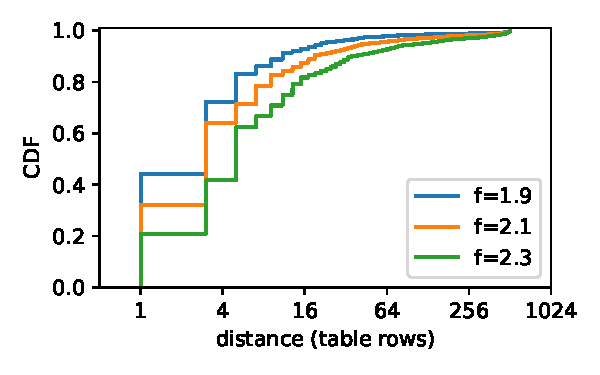
\includegraphics[width=0.99\linewidth]{fig/hash_factor.pdf}
        % \label{fig:hash_factor}
        % \caption{}
    \end{subfigure}
    \begin{subfigure}{0.3\linewidth}
        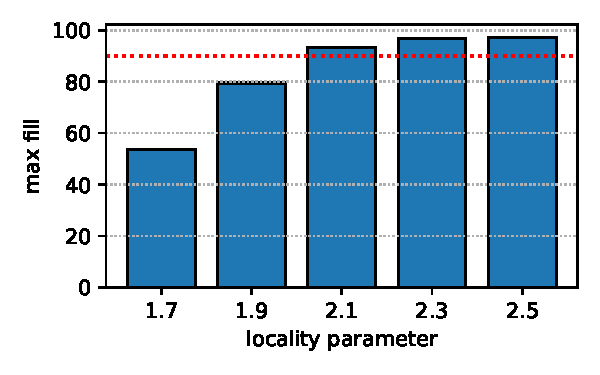
\includegraphics[width=0.99\linewidth]{fig/hash_fill.pdf}
        % \label{fig:hash_fill}
        % \caption{}
    \end{subfigure}.
    \vspace{-1em}
    \caption{
    \textbf{(a)} Dependent hashing for factor $f$.
    \textbf{(b)} CDF of distances between cuckoo locations dependent hashing on different exponential factors.
    \textbf{(c)} Exponential factor relation to max fill in cuckoo hash. 90\% fill marked in red.
    }
    \label{fig:locality-hashing}

\end{figure*}




\subsection{Dependent Hashing}

Our hashing algorithm borrows from both cuckoo and hopscotch
hashing to achieve constant time reads and a high degree of
locality. The distance between two hash locations is
determined by probabilistically \textit{dependent} rather
than independent hash functions. Dependence makes locality a
tunable parameter. High locality increases the probability
that a single RDMA read can capture both hash locations and
decreases the number of locks required for updates. High
locality increases the chance that an insertion operation
will fail, decreasing the max fill of the table.

Figure~\ref{fig:locality-hashing}(a) is the formula for dependent
hashing. The first hash location is chosen uniformly at
random, while second is chosen as an offset of the first.
$f$ determines the max distance the second item can be
placed. Higher values of $f$ decrease locality.
Figure~\ref{fig:locality-hashing}(b) shows the distance between hash
locations as a CDF for different values of $f$. Setting a
constant bound on the distance between hash locations leads
to bad fill factors (on the order of 10-15\%). Our function
places exponentially few locations exponentially far apart
using a third hash function $h_3(x)$ which generates a
higher exponent at a logarithmic rate to determine which
locations will have large distances between
them~\footnote{The value of $h_3(x)$ is the sum of trailing
zeros after calculating a keys 64bit hash value} These few,
but far apart hash locations increase the max fill by
alleviating hotspots in the table. During inserts these
entries act as gateways for search to access less filled
portions of the table. 

Figure~\ref{fig:locality-hashing}(c) shows how larger values of $f$
enable higher fill factors for tables with 100M entries.  In
our experiments we use $f$ of 2.1 and an associativity of 8
as it provides a 90\% max fill an a 68\% probability that
hash locations are located 3 or fewer buckets apart.


% in a single RDMA read, and
% that fewer locks are required while performing updates.

% the constant time reads of
% cuckoo hashing with the locality properties of hopscotch
% hashing. Traditional cuckoo hashing requires two independent
% hash functions which set key locations uniformly at random.
% We use two ~\textit{dependent} hash functions to increase
% locality between key locations. The first hash function
% selects a row in the cuckoo table uniformly at random. The
% second second hash function selects a location randomly from
% the following $n$ rows after the first hash location. The
% value of $n$ is not constant. A third hash function $h_3(x)$
% generates values of $n$ according to an exponential
% distribution. We use a constant factor $f$ to control the
% exponential function.  Figure~\ref{fig:locality-hashing}(a)
% shows the formula for our dependent hash functions.

% The constant value $f$ determines the distribution of
% distances between key locations.
% Figure~\ref{fig:locality-hashing}(b) is a CDF of distances
% between key locations for 3 values of $f$. A distance of 1
% means that a keys second location is in the row immediately
% after it's first location. In the case of $f$=2.3 20\% of
% keys have a distance of 1 bucket. Small values of $f$ have
% high locality. However, locality is not free. Independent%%
% hash functions enable cuckoo hashes to read high fill rates (95\% and higher).
% %%
% Removing independence increase the probability of
% hotspots which cause insert operations to fail. A cuckoo
% insertion fails if no sequence of swaps exists which can
% produce a valid cuckoo path. Failed insertions require the
% table to be resized and directly effect memory utilization.
% Therefore $f$ is directly related to the maximum fill factor
% a table can achieve using dependent hashing.

% An over
% filled region of the table can quickly lead to deadlocks
% when inserting requiring the table to be resized. $f$ is
% directly related to the max fill factor of the table. Larger
% $f$ values increase the max fill factor, while decreasing
% locality.  

% Figure~\ref{fig:locality-hashing}(c) shows the relationship
% between $f$ and a tables maximum fill. These values were
% generated by inserting into a cuckoo table with 100M entries
% until an insertion failed. Table associativity directly
% effects fill rate. The higher the degree of associativity
% the more likely a valid path will exist. The table used in
% Figure~\ref{fig:locality-hashing} has an associativity of 8
% similar to prior cuckoo
% hashes~\cite{memc3,cuckoo-improvements,pilaf}.


% The associativity of the
% cuckoo hash plays a key role in enabling high fill. The
% higher the degree of associativity the greater degrees of
% freedom search is given to escape local hotspots.

%The second hash function determines the maximum
%distance the second value can have from the first. A third
%hash function determines a random location between the first
%location, and the bound imposed by the second.
% Figure~\ref{fig:locality-hashing}(a) shows the formula for our hashing
% function process, which implements the probabilistic region-size
% selection with a third hash function---akin to the way Bitcoin
% computes its difficulty.
% \textbf{Why not make the second hash function a true expoential?}

% A strawman implementation of locality based hashing would
% use the first hash function to find a location, and the
% second to find a random location within a fixed bound. This
% approach quickly leads to failed insertions. Due to the
% birthday paradox the probability of a collision is high, and
% on large tables the probability that one region of the hash
% table will become full, and have not viable path to an open
% slot is high. ~\sg{Perhaps this justifies a figure, please
% advise.}.

% We use a dynamic exponential bound rather than a static one.
% The dynamic bound is set by raising a constant factor $f$ by
% an exponent determined by a third hash function. Using the
% third hash on the key we count the number of suffix zeros
% and raise the constant factor by itself plus the zero count.
% This distribution generates exponential distances between
% hash locations at exponentially less frequency and is
% tunable with the single parameter $f$.
% %%
% In the common case the bound is small. Exponentially few key
% are spaced far apart and act as~\textit{waypoints} to other
% regions of the table when constructing cuckoo paths. This
% method, paired with bucket associativity enables high fill
% rates while keeping the region of the table any given key
% can inhabit small.

% There is a tradeoff between locality and fill factor.
% Figure~\ref{fig:locality-hashing}(b) illustrates how
% increasing the exponential factor shifts the distribution of
% distances between cuckoo hash locations.
% Figure~\ref{fig:locality-hashing}(c) shows how these same
% factors effect the max fill rate of the table before an item
% cannot be inserted. As will be shown in the following
% sections read, and insert performance improve with better
% locality. Therefore fill factor and performance can be
% traded off directly by changing the exponential factor. In
% our evaluation we found an exponential factor of 2.3 to give
% the best results in terms of end to end performance and
% bandwidth consumption.


\subsection{Locking}
\label{sec:locking}

\begin{figure*}[t]
    \centering
    \begin{subfigure}{0.3\linewidth}
        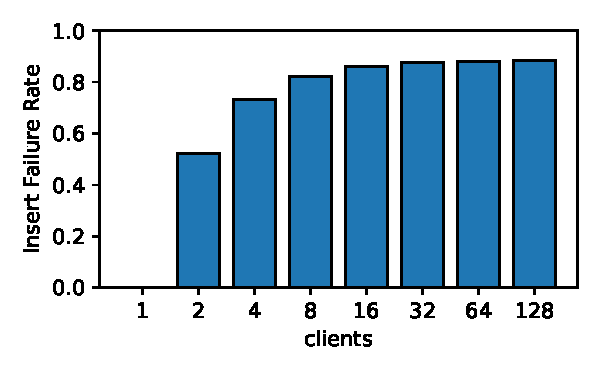
\includegraphics[width=0.99\linewidth]{fig/optimistic_failures.pdf}
        % \label{fig:optimistic_failures}
        % \caption{}
    \end{subfigure}
    \begin{subfigure}{0.3\linewidth}
        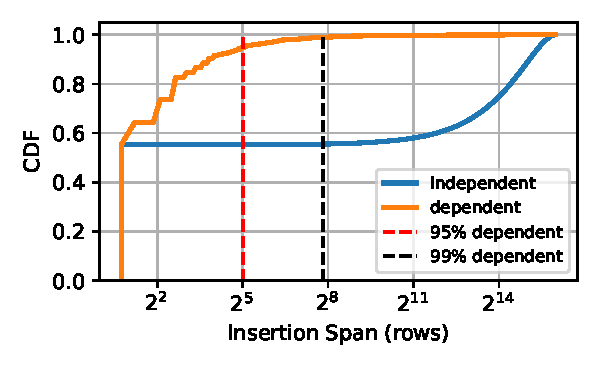
\includegraphics[width=0.99\linewidth]{fig/insertion_span.pdf}
        % \label{fig:insertion_span}
        % \caption{}
    \end{subfigure}
    \begin{subfigure}{0.3\linewidth}
        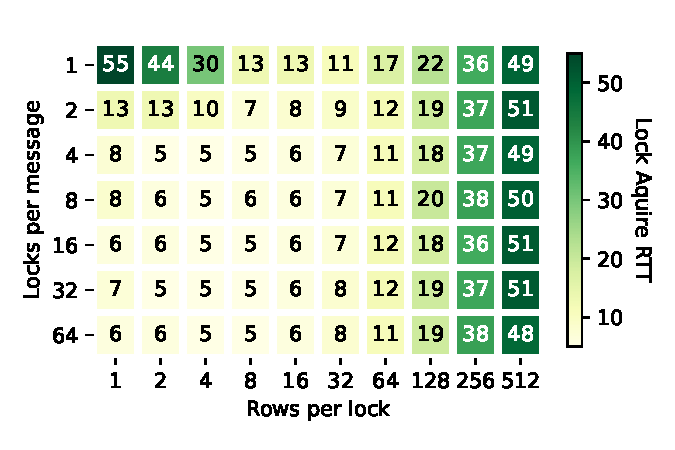
\includegraphics[width=0.99\linewidth]{fig/buckets_per_lock_vs_locks_per_message.pdf}
        % \label{fig:tbd}
        % \caption{}
    \end{subfigure}
    \vspace{-1em}
    \caption{
    \textbf{(a)} Failure rate of optimistic cuckoo insertions.
    \textbf{(b)} CDF of cuckoo spans for dependent and independent hashing. A cuckoo span is the distance between the smallest and largest index in a cuckoo path.
    \textbf{(c)} Round trips (99th percentile) on a table
    with 512 rows required per insert while filling a table
    to 95\%. 512 buckets per lock is a single global lock.}

    \label{fig:cuckoo-problems}

\end{figure*}

Using locks rather than opportunistic concurrency halves the
latency of reads from two to one round trip. Opportunistic
updates commit changes by atomically updating a pointer
(with CAS) in the hash index to point to a new value. Both
the index, then the value must be read for each operation.
Values can not be inlined in the index as they are limited
to the 64bit width of CAS. Rcuckoo uses locks to enable
inlined entries which can be read in a single round trip.
Locks introduce multiple challenges such as scalability,
deadlocks and fault tolerance each of which is discussed
below.

RCuckoo uses hardware NIC hardware features and lock
virtualization to achieve scalability, low contention and
high performance. The lock table is a linear array of bits
where 1 is locked, and 0 is unlocked. Each bit locks one or
more contiguous rows in the table. In our experiments we use
16 rows per lock as it has a negligible effect on contention
and requires a single lock to be acquired for \todo{85\%
double check} of insertions.

We use two RDMA NIC features to accelerate lock
acquisition. First the lock table is placed in NIC device
memory which allows atomic operations (CAS) to
scale linearly with reads and writes and is 3x higher
throughput on contented addresses than host memory (see
Figure~\ref{fig:rdma-benchmarks}). It is also lower latency
as operations to device memory avoid a PCIe round trip.
Second, RDMA Masked Compare and Swaps (MCAS) are used rather
than CAS~\cite{rdma-masked-cas,sherman}. CAS requires an
exact 64 bit match to execute, while MCAS uses a mask to
only set the required bits. MCAS therefore reduces
contention while enabling locks to be as tightly packed.

Packing locks densely is important as NIC device memory is
limited to 256KB which by default limits table size. We use
a \textit{virtual lock table} to avoid limiting table size
by device memory.  Multiple virtual locks map to a single
physical lock. We use modulo arithmetic to map virtual locks
onto physical lock to support arbitrarily large tables.
Mapping multiple virtual to a single physical lock leads to
false sharing, clients can be blocked unessisary on a lock.
In Section~\todo{TODO} we show that on large lock tables the
performance degradation due to false sharing is low, and
that lock locality is maintained on virtual locks.

% Our lock table is an array of contiguous bits where each bit
% is a lock, and each lock guards one or more sequential
% buckets. The size of the lock table in bytes equals the
% number of hash table rows, divided by the number of rows
% each lock guards (rows per lock). The size of a lock table
% for a cuckoo table with 100M entries, 8 entries per row, and
% 16 rows per lock is 102KB.  Lock table size, and rows per
% lock are important variables as they enable us to utilize
% two features of modern RDMA NICs, mainly device mapped
% memory, and masked compare and
% swap~\cite{rdma-masked-cas,sherman}.

% Device mapped memory is a small region of on NIC memory,
% typically on the order of 256KB. This memory executes
% one-sided RDMA operations faster than host memory as the
% operations need not make a PCIe round trip. This memory is
% especially performant for atomic operations as the NIC would
% otherwise have to queue dependent atomic request to host
% memory. Figure~\ref{fig:rdma-benchmarks}(c) shows the
% performance boost from device over host memory for atomic
% operations.

% Disaggregated indexes may be very large, and require more
% than 256KB of device mapped memory to store an entire lock
% table. To enable lock tables larger than device device
% memory can hold by default we implement a \textit{virtual
% lock} table. 

% Multiple virtual locks map to a single physical
% lock. We use modulo arithmetic to map virtual locks onto
% physical lock to support arbitrarily large lock tables.
% Mapping multiple virtual to a single physical lock leads to
% false sharing, clients can be blocked unessisary on a
% lock. In Section~\todo{TODO} we show that on large lock
% tables the performance degradation due to false sharing is
% low, and that lock locality is maintained on virtual locks.

% The second NIC feature we exploit is masked compare and swap
% operations. Masked cas operations enable clients to set
% individual bits rather than 64 bit spans. As our lock table
% is tightly packed this enables clients to aquire locks
% without any additional knowledge about the lock table as
% would be required for unmasked cas.

Our deadlock free locking protocol acquires and releases
locks in order.  Given a list of virtual locks to aquire a
client calculates their physical locations and sorts them.
The sorted locks are broken into 64 bit chunks which are
mapped to individual MCAS packets. As shown in
Figure~\ref{fig:cuckoo-problems}(b) 99\% of insertions are
within a 256 bucket range. Each MCAS covers 1024 buckets so
the common case is a single chunk. Lock requests are issued
in order. Clients continuously poll on lock requests and
only move to the next request only after the prior has been
successfully acquired.

Clients may fail while holding locks leaving them set and
stranded. Clients detect failed locks by timing out on them
while acquiring them. To separate failures from clients
acquiring a long list of contended locks clients are given a
bounded time to aquire their locks. If a client takes longer
than this time to aquire all of its locks it releases all
held locks and starts the process again to prevent false
failure detection. Our complete fault detection and recovery
mechanism is described in Section~\ref{sec:fault-tolerance}.

% Together with locality hashing these features enable the
% following fast locking protocol. When a client requires
% locks it calculates all lock indexes locally by performing a
% local search. Lock indexes are the row the client must lock
% divided by the number of rows per lock modulo the size of
% the physical lock table. Once the set of locks is calculated
% the client breaks the set of locks into separate locking
% requests. If the locks are within 64 entries of each other
% all locks are packed into a single masked compare and swap
% packet. If the span of locks is greater than 64 a second
% packet is generated with all locks in the next range of 64
% packed together into a single packet.

% Deadlocks are avoided by acquiring locks in a global order
% from smallest to largest. This is done by sorting the locks
% after the virtual to physical mapping occurs. Locks are
% released in the same order. If the locks a client acquires
% are not sufficient to complete it's operation it releases
% the locks and tries again.

% We use RDMA device memory for our lock
% table~\cite{rdma-masked-cas}. To aquire locks clitnts
% locally determine which locks they require for their
% operation, and then issue RDMA masked CAS operations to the
% device memory. This approach enable clients to aquire up to
% 64 contiguous locks with a single RDMA operation and enable
% clients to aquire locks without synchronizing the state of
% the lock table prior to acquisition (non masked CAS would
% need the state of all locks prior to issuing the request.).

% This locking scheme in conjunction with dependent hashing
% enables most client operations to aquire locks in a singe
% round trip. Update and insert operations require at most two
% locks, one for each key location. Using $f$ of 2.3 90\% of
% key pairs are within 64 rows of each other so even with row
% per lock 90\% of updates and deletes can be completed in two
% round trips. In practice we use 16 rows per lock which
% results in 99.7\% of updates and deletes resulting in two
% round trips.

% Inserts can span arbitrary regions of the table and are a
% harder case than updates and deletes.
% Figure~\ref{fig:cuckoo-problems}(b) shows the span in rows
% of cuckoo paths for a table with 100K rows. These spans are
% the difference between the highest and lowest row locked
% during insertion. Using dependent hashing 95\% of insertions
% span 32 rows or less, and 99\% of insertions span 256 rows
% or less. Using 16 rows per lock each masked cas can cover
% 1024 rows of the table ensuring that 99.5\% of insertion
% locks can be acquired in a single round trip.

% Using this locking scheme locality hashing greatly improves
% locking performance. With independent hashing the locks for
% a cuckoo path are scattered randomly throughout the table.
% Therefore, a round trip is required for each lock, and each
% lock must be acquired in order to avoid deadlock. With
% locality, and the ability to lock up to 64 sequential locks
% most insertions can be performed with a single round trip
% for locking. In both cases lock release can be batched in a
% single round trip.

% Figure~\ref{fig:cuckoo-problems}(b) shows the insert span in
% buckets using both dependent and independent hashing on a
% table with 500K entries and an associativity of 8. A span is
% calculated as the distance between the lowest index and the
% highest index in a cuckoo path. Past 50\% independent
% hashing spans a random range in the table (whenever a
% displacement occurs on insert). With dependent locality
% based hashing 95\% of inserts span less than 32 buckets, and
% 99\% less than 256.


% Traditional wisdom would suggest that because cuckoo hashing
% can have long insertion paths it is a poor candidate for
% remote memory. Both opportunistic, and lock based approaches
% have significant drawbacks.
% %%
% As an example consider an opportunistic approach in which
% many clients are inserting concurrently to a table. Clients
% making inserts first make reads of the table to locally
% calculate a cuckoo path for their insertion. After the reads
% complete the client constructs a cuckoo path and starting
% from the open slot issues dependent CAS requests migrating
% the open slot backwards to the insertion bucket.
% %%
% Figure~\ref{fig:cuckoo-problems}(a) shows the failure rate
% of this insertion scheme as a factor of clients running
% inserts on a table with 500K entries with a bucket
% associativity 8. Cuckoo paths calculated from client caches
% quickly become invalid as the number of clients grows.
% %%
% Alternatively deadlock free lock acquisition requires more
% round trips and has larger critical sections. Each lock must
% be acquired in order with a dependent CAS request which
% incurs an additional round trip per lock. Using course
% grained locks reduces the number of acquisitions but
% throttles throughput as concurrent insertions are more
% likely to contend shared locks.

% Locality hashing increases the probability that an insertion
% path is within a small region of the hash table which in
% turn increases the probability that fine grained locks will
% be near one another. 
% %%
% Figure~\ref{fig:cuckoo-problems}(b) shows the insert span in
% buckets using both dependent and independent hashing on a
% table with 500K entries and an associativity of 8. A span is
% calculated as the distance between the lowest index and the
% highest index in a cuckoo path. Past 50\% independent
% hashing spans a random range in the table (whenever a
% displacement occurs on insert). With dependent locality
% based hashing 95\% of inserts span less than 32 buckets, and
% 99\% less than 256.
% %%
% RDMA masked CAS operations allow a client to set a 64 bit
% mask along with the new, and old values of the cas
% operation. So locks can be acquired with minimal knowledge
% of the remote lock table. This enables the client to
% atomically set up to 64 contiguous locks independently which
% dramatically reduces the round trips required to aquire
% locks.

% Lock granularity effects performance under contention. Using
% values from Figure~\ref{fig:cuckoo-problems}(b) if locks are
% per bucket 96\% of lock acquisitions can be completed with a
% single RTT masked cas. If locks span 4 buckets 99\% of
% requests can be completed in a single round trip.

% Increasing the number of buckets each lock guards can reduce
% the number of locks required for an operation.
% Figure~\ref{fig:ycsb_fill_latency}(c) shows the tradeoff
% between lock granularity and the number of locks which can
% be set in a single message with locality hashing turned on.
% The table has 512 rows total to illustrate the effect of a
% single global lock.

% The values
% reported are the 99th percentile number of round trips
% required to acquire locks up to a 90\% fill factor on a
% table with 4096 entries and 8 entries per bucket, and 8
% concurrent clients. The biggest factor in round trip times
% is the number of locks per bucket. On the far right side of
% the heatmap (512) only a single global lock exists. Further
% the benefit in terms of locks per message falls off quickly
% after two. RDMA-masked CAS are beneficial as they allow for
% fine-grained locking, but setting 3 or more locks per
% message has little effect up to 90\% fill rate. Reducing
% atomic operations in turn reduces the effect of the RDMA
% atomic bottleneck.  \textbf{Hard to see 3; the figure only shows 2 or 4.}

% Our lock table is small in comparison to the true hash
% table. At its most fine-grained each lock corresponds to
% one bucket (8 entries). Each lock is 1 bit, a lock table for
% a 100 million entry hash table is ~160KB, with a lock
% granularity of 4 buckets this drops to 40KB. This tight
% layout enables us to use device-mapped memory to hold our
% lock table~\cite{design-guidelines,sherman}.
% %We make use of
% Device-mapped memory on recent RDMA NIC's (ConnectX-5+) avoids an
% expensive PCIe round trip, reducing lock acquisition latency.
% This enables up
% to 3$\times$ better throughput on contested locks (see
% Figure~\ref{fig:rdma-benchmarks}(c)), and reduces latency
% for locking.

\subsection{Table Design}

Our table is designed to facility fast reads as they are the
dominant operation for key value stores in data
centers~\cite{facebook-memcached}.
Figure~\ref{fig:table-diagram} illustrates our tables
two-part design in the midst of an insertion for key $K$.
~\todo{update diagram} The lock table
(Section~\ref{sec:locking}) is shown on the left~\todo{add
virtual table}. The table index (right) is a single
contiguous array of bytes allocated at initialization time.
Both the table size, and entry size are set
statically~\todo{We leave resizing to future work.}. 

Each row contains $n$ entries and terminates with an 8 bit
version number and 64 bit CRC. Inlined table entries begin
with a 0 bit and keep all data in the index. RCuckoo also
supports extent entries for large values~\footnote{Inlined
entries perform better on small key value pairs} where table
entries point to out of index extent values. On updates
clients modify an index entry then increment the row version
number and recalculate the rows CRC including the version
number. CRC's enable lockless reads as each row can be self
verified. Version numbers ensure clients polling for locks
can differentiate between highly contested locks and clients
that have failed while holding locks (Section
~\ref{sec:fault-tolerance}).


\subsubsection{Client Caching}

Rcuckoo clients keep caches of the remote index locally.
During insertions caches are used to perform local searches.
Caches can be purged between requests to save space on the
client or persisted between requests to aid in predicting
future search paths. Our experimentation shows that lock
granularity paired with covering reads
(Section~\ref{sec:insert}) has a far higher impact on search
success over caching (Section~\ref{sec:search_success}) as
index state changes rapidly under load.

\subsubsection{Memory Allocation}
%%
\sg{Help alex, I need to remove this section but I don't
quite know how to talk about memory allocation or extent
memory}
%%
Prior work has focused on different memory allocation and
hash table resizing schemes. Sherman~\cite{sherman} uses an
allocated thread located on the memory node,
Fusee~\cite{fusee} uses a two tired memory allocation in
which large blocks of memory are allocated on the memory
nodes and fine grained allocation is performed on the
clients. Clover~\cite{clover} statically partitions memory
into large client regions prior to execution and hash
clients entirely manage the space themselves. Network based
allocators such as MIND and Clio~\cite{mind,clio} have
demonstrated the feasibility of high performance
disaggregated allocators, while some have called for
allocators to be built into RDMA~\cite{prism}. We allocate
memory using the same scheme as Clover, as it is simple to
implement and adds no additional overhead. We view memory
allocation as a hard orthogonal problem to the design of
disaggregated indexes and have designed our system
acrostically to the allocator.




\begin{figure}[t]
    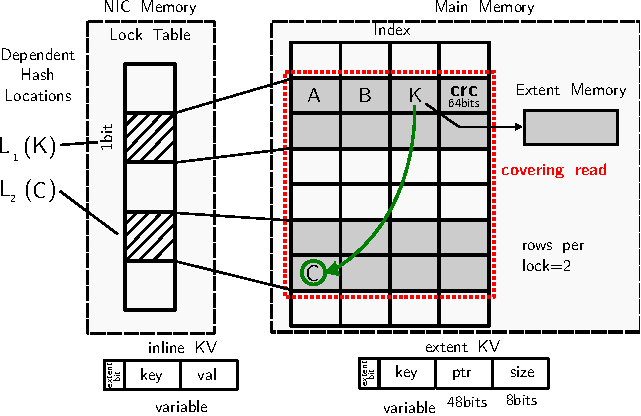
\includegraphics[width=0.99\linewidth]{fig/table-diagram.pdf}
    \caption{Rcuckoo's table design showing an insert of the key $K$ as it displaces $D$.}
    \label{fig:table-diagram}
\end{figure}


\subsection{Protocol}

\begin{figure}[t]
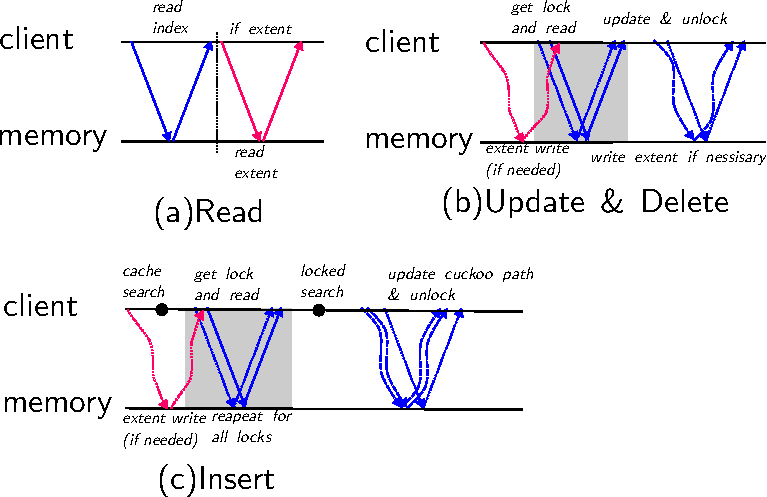
\includegraphics[width=0.99\linewidth]{fig/message_diagram.pdf}

\caption{Rcuckoo's protocol for reads, inserts, deletes and
updates. Blue lines are index accesses, and red lines are
extent accesses. Solid lines are reads, dotted lines are
CAS, and curved dashed lines are writes.}

\label{fig:message_diagram}
\end{figure}

In this section we describe our protocol for reading,
inserting, and performing updates and deletes to an rcuckoo
hash table. Figure~\ref{fig:message_diagram} visualizes our
protocol.

\subsubsection{Reading} 
\label{sec:reading}

Read requests for key $K$ start by hashing $K$ to calculate
both row locations. Reads are combined if both rows are
within a read threshold to reduce tail latency. We use a
read threshold of 128 bytes as it has a negligible increase
in latency over smaller RDMA
packets~\ref{fig:rdma-benchmarks}(a). If reading both
locations as a single read is greater than 128 bytes, the
read is issued as two parallel reads to individual rows
similar to prior work without locality
optimizations~\cite{pilaf, race}. Inlined entries are read
in a single round trip, while extent entries require two
(Figure~\ref{fig:message_diagram}).

Reads are performed locklessly. Readers recalculate and
check the rows CRC to validate the read. Clients reissue the
read if the CRC is invalid as it is likely due to the read
encountering a torn write. Continuously invalid CRC's can be
the result of a client failure mid write. Our algorithm for
detecting and repairing the table from partially completed
writes is described in Section~\ref{sec:table-repair}.

% If key-value entries are inlined reads complete in a single
% round trip. Larger key stored in extents require a second
% round trip as clients must first read the index, resolve the
% virtual address of the extent and then perform the extent
% read.
% %%
% ~\footnote{This design requires exactly one pointer
% resolution in expectation that future RDMA NICs may provide
% pointer resolution reads as a primitive~\cite{prism}}
% %%
% Reads are lockless and can see partially completed writes.
% We use a 64 bit CRC to check read
% validity~\cite{pilaf,cell}. Unlike prior approach we use a
% single 64bit CRC per table row, rather than per entry. This
% approach reduces per entry CRC overhead in the index.
% %%
% We define a read threshold of 512 bytes for our clients.
% Approximately 60\% of keys for 64-bit entries with a bucket
% size of 8 (see Figure~\ref{fig:locality-hashing}(b)) fall
% into this category. This has the advantage of updating the
% client cache for future operations.
%, and reduces the header processing required by the NIC.
% To reduce bandwidth the size of the threshold can be tuned
% down, or turned off with no harm to correctness.

% \subsubsection{Locking and unlocking}

% Update, delete and insertion operations all require locks to
% modify the index. Locks are acquired in incremental order
% from smallest to largest to avoid deadlocks. First the list
% of locks required for the operation is calculated. For
% updates and deletes two locks may be required. Inserts may
% required many locks. The client calculates which locks it
% requires and breaks the list into masked CAS operations
% spanning 64 locks and then issued the requests polling for a
% successful response before moving to the next lock.

% To synchronize the client cache with remote memory we issue
% a \textit{covering read}. A covering read is an RDMA read
% which spans the range of buckets from the lowest lock in the
% masked CAS to the highest. The covering read is issued after
% the masked CAS and ensures the client receives synchronized
% data for the locked buckets while not consuming an
% additional round trip.

% Clients need their caches synchronized with remote memory
% prior to modifying it with writes. We batch reads with lock
% requests to synchronize client caches. RDMA in-order
% delivery ensures that reads issued after a lock request will
% be up to date, as no other client can concurrently modify
% the locked index.  A spanning read is issued for each lock
% request. The read covers each bucket the client locks.  For example, if a
% masked CAS has three locks, reads are calculated for each
% bucket being locked. If the locks cover a range less than
% the read threshold a single read is issued which spans all
% buckets between the locks.  Spanning reads are issued concurrently with
% lock requests.
%Subsequent lock requests are issued prior to
%blocking on reads.

% After locks are acquired the client can execute its critical
% section. Unlock requests are the inverse masked CAS operations of the
% lock requests. Clients issue their critical sections as a sequence of
% (asynchronous) writes followed immediately by unlock operations. RDMA
% in-order delivery ensures that the unlock operations are performed
% after the writes.

\subsubsection{Updates and Deletes}

Updates and deletes use an identical message protocol. They
first get both locks for key $K$ while issuing covering
reads (Section~\ref{sec:locking}). If the key is present the
entry is either updated or deleted the version number for
the row is updated and a new CRC is calculated. Both
modifications are issued as separate RDMA writes. For extent
updates new values are batched along with lock requests
preventing an additional round trip. Extent deletes mark the
extent entry for garbage collection.

% are similar operations as both require
% two locks. In the locking phase clients calculate and aquire
% both locks (Section ~\ref{sec:locking}). Updates to inlined
% entries issue a single entry sized update directly to the
% index. The row version number is incremented and a new CRC
% is calculated for the updated row and bached along side the
% update or delete.  Updates to extents issue three messages
% first the new extent is written, the index is updated, and
% finally the old extend is set to invalid and marked for
% garbage collection. In both cases unlock messages are
% batched with the update. Similarly deletes lock both table
% entries. On deletes clients compact the row so open entries
% are always located at the end of the row~\footnote{Ensuring
% open entries are at the ends of rows improves search times
% for open buckets.}. Extent entries are marked as invalid in
% the same round trip. Both updates and deletes commonly
% execute in 2 round trips. 3 round trips are required only if
% both locks are too far apart to be set in a single masked
% cas operation.

\subsubsection{Insert}
\label{sec:insert}

Insertions are the highest complexity operation because
client caches are not synced with remote memory. Without
knowing the state of remote memory clients can neither
calculate valid cuckoo paths locally and nor determine which
locks they will require to perform an insertion. We uses a
speculative local search to predict a sufficient set of
locks to complete the insertion and then lock and
synchronize the predicted rows. A second search on the
locked and synchronized rows determines if a valid insertion
path can be found on the locked rows.

\textbf{Speculative Local Search:} The first stage of an
insertion is a speculative local search on the clients
cache. If the client cache is empty a lock for both of the
insertion keys hash locations are made. Otherwise, locks for
each row on the speculative path are acquired. Because of
locality hashing there is a high probability that a valid
insertion path can be found in buckets near a speculative
path, even if the clients cache is stale.

\textbf{Covering Read:} Clients synchronize their local
caches while acquiring speculative locks by reading the rows
the lock protects. These reads are issued in a batch
alongside the MCAS lock request. Speculative locks may not
be sufficient to complete an insertion. However, due to
locality hashing there is a high probability that a valid
path does exist in the neighborhood of the speculative
locks. If two speculatively locked rows are close enough
together clients issus a single \textit{covering read}
spanning both rows. Covering reads populate a clients cache
and dramatically increase the probability that if the first
speculative search fails, a subsequent search will succeed.
We set the max threshold for covering reads to 512 bytes in
all our experiments.  Figure~\ref{fig:table-diagram}
illustrates an insertion of key $K$ displacing key $C$. Here
the speculative search marked the rows for $C$ and $K$ to be
locked. A covering read (red) spans the rows between both
entries.

\textbf{Second Search:} A speculative cuckoo path may be
invalid due to churn in the index. However, as noted their
is high probability that a valid path can be found within
the locked rows due to hash locality. Clients perform a
second search only on the synchronized rows that they have
locked. We use BFS similar to prior work, as it produces
short paths which minimize bandwidth and locking
overhead~\cite{cuckoo-improvements}. If a valid cuckoo path
is found during second search each update and CRC along the
path along with unlock messages are batched together. If no
valid path exists the client releases its locks but retains
its cache. Another speculative search on the fresh cache is
performed. This algorithm is run itteratitivly until a valid
path is found. Our evaluation measures the success rate of
insertions as a factor of lock size
(Section~\ref{sec:search_success}).

During development we
experimented heavily with guided A* search but found that it
only offered improvements over BFS when the table was over
95\% full due to the setup overhead of A* and the fact that
most paths are short.

% The speculative path may not be
% valid after clients have acquired locks and synchronized
% their caches. If the speculative path is not valid clients
% perform a second search restricted to the rows locked by the
% client. Due to dependent hashing cuckoo paths are highly
% localized. If locks cover 8 or more rows clients have a high
% probability of constructing a valid cuckoo path using the
% rows locked by their first search. If clients can not find a
% valid path with their second search the client releases it's
% locks and tries again. Subsequent searches have a high
% likely hood of success as clients retain their caches across
% requests. We measure the success rate of second searches in
% response to the number of rows per lock in our evaluation
% (Section~\ref{sec:search_success}).

% Cuckoo paths and updates are issued in a single batch. If a
% valid search path is found path updates are made as a batch
% of sequential writes. Unlock operation are batched after the
% writes. Writes to the extent precede updates to the table.
% Insertions are the most expensive operation as they require
% computation, large reads, and writes. In our evaluation we
% find that insertions are limited by the network bandwidth of
% our CX5 NIC's not lock contention or failed searches. We
% consider this a desirable limitation as network bandwidths
% continue to increase and so additional operation throughput
% can be exchanged for additional bandwidth~\footnote{CX7
% NIC's currently support 400Gbps line rate.}.


% \subsubsection{Search Algorithm} 

% Cuckoo paths are highly influenced by the search algorithm 
% used to find them. Prior work has used DFS to construct 
% cuckoo paths~\cite{pilaf,memc3}. We follow prior work and 
% use BFS as it produces the shortest 
% paths~\cite{cuckoo-improvements}. Short paths reduce the 
% number of locks required. Dependent hashing opens new 
% opportunities for search optimization as open slots are more
% likely to be close to an initial hash location. As part of
% our work we investigated using guided search A* to construct
% short paths using locality information. We found that A*'s
% performance only improves on BFS at fill rates about 95\%
% which are rarely found in practice due to max fill rate
% limitations.

\subsection{Fault Tolerance}
\label{sec:fault-tolerance}

Prior disaggregated data structures have achieved client
based fault tolerance by committing changes to data
structures with a single atomic CAS~\cite{clover,race},
while lock bases systems have not handled client
failures~\cite{sherman}. The key challenge in handling
client failures is recovering when a client dies while
holding one or more locks. A failed client with a lock may
have incomplete writes leaving the table in an inconsistent
state. Furthermore, detecting client failure and
relinquishing locks is hard as a failed client may have
issued writes which could be delivered to memory after the
lock has been revoked. In this section we describe our
failure detection method, how we protect memory from errant
writes, and how we recover from partially completed operations.

\subsubsection{Failure Detection} We detect client failures
using timeouts. Clients start timers when they either fail
to complete a read due to an inconsistent CRC or when they
fail to aquire a lock. Once a client starts a timer it
repeats its request continuously until it's failure timeout
fires. Failure to read an entry, or obtain a lock may be the
result of contention. A heavily contested lock may take a
long time to aquire via attempted CAS requests.
Simultaneously reads may fail due to seeing different
partial updates to the table. We enable clients to
differentiate between contention and failure by adding an 8
bit version counter to each row in addition to the 64 bit
CRC. When clients update a bucket they increment the rows
version number prior to calculating the CRC64 of the row.
Version numbers cause the CRC to change on each update. When
clients note that a rows CRC has changed they reset their
fault detection timer. Only when a client has attempted to
aquire a lock or read for the full duration of the fault
timer and the table has not changed does the client flag the
fault as valid.

During insertions clients can require many locks, and
therefore hold locks for arbitrary time during their
acquisition. We bound lock acquisition time so clients can
detect failures. Clients which take too long to aquire their
locks release all their locks, and recalculate their
insertion paths.  We set our failure timeout to \todo{2x
(ora constant multiple of)} our lock acquisition timer.

\subsubsection{Lock Reclamation} Once a client has detected
a failure it reclaims the stranded lock and if unessisary
repairs the table. The most basic failure condition is that
a client fails prior to releasing the lock but has left the
table in a valid state. In this case the repair client
acquires a repair lease for the table, and then issues a
masked cas to unlock the timed out lock. Repair leases are
separate locks from the lock table. When a client aquire a
repair lease it set it with a lock bit, it's queue pair id,
and a counter. The counter is incremented each time the
lease is acquired or released. The purpose of the repair
lease is to ensure that no more than one client attempts to
repair the table at the same time. Failure timeouts on
repair leases are similar to table based timeouts, except
that clients can determine if the lease has changed hands
simply by reading it. Rcuckoo supports multiple repair
leases so that table repairs can be run in parallel. Each
lease spans a range of physical locks. Clients calculate
which lease or leases they require based on the locks they
are reclaiming. Once a client has repaired the table and
reclaimed the lock in question it releases the lease.

\subsection{Table Repair} 
\label{sec:table-repair}
Cuckoo updates occur along a path
and client failures could occur at any point along an
insertion path. Updates and Deletes are a special case where
the path length is 1. If a client fails mid modification it
can leave the table in 3 distinct states based on where in
the update it fails. Cuckoo insertions migrate an open slot
back to the bucket the insertion must occur in. When
propagating along a path. Clients write a duplicate entry,
then update that duplicates CRC, then move on to the next
entry removing the duplicate by overwriting the next entry
on the path. The three distinct incorrect states are as
follows 1) The table contains a duplicate entry, and one of
those entries has an incorrect row CRC. 2) The table
contains a duplicate entry and both entries have correct
CRCs. 3) The table does not contain duplicates but one row
has a bad CRC. Repairing clients must detect which state the
table is in and then repair the table in a deterministic way
so that if they fail during repair subsequent clients can
repair their failed attempts.

Prior to acquiring repair leases a client first performs a
series of reads. First it reads all buckets protected by the
lock it timed out on. Then it iterates through each entry in
every bucket checking the table for duplicates on each
entry. The repair client can detect which state the table is
in by detecting duplicates and checking the CRC on each row.
If duplicates exist, and a row has a bad CRC the table is in
state 1) if a duplicate exists and the CRC's are good the
table is in state 2) and if a row only has a bad CRC the
table is in state 3). Once the client has determine which
state the table is in it aquire a repair lease for those
rows. After acquiring the lease the client rereads the rows
to ensure they were not corrected by another client before
proceeding. 

The repair is performed by issuing a deterministic set of
writes to transition the broken rows through each state. To
transition from state 1) to state 2) the client recalculates
the CRC of the row with a broken CRC and issues the write
placing the table in state 2). To transition the table from
state 2 to 3 the client must make a deterministic choice.
The repair client has no knowledge of the original operation
so it complete the operation by simply removing one
duplicate. In this case it always removes the duplicate in
the secondary cuckoo location. By writing an empty entry to
the second entry location the table is transitioned into
state 3). State 3 is repaired by recalculating and writing
the CRC for the inconsistent row. Post repair only locks
need to be released. This method enable any client to repair
the table and to fail during any stage of the repair while
allowing other clients to finish the repair.

\subsubsection{Preventing Stale Writes}

Revoking a lock does not prevent writes from being issued
directly to memory. If a client issues a write an fails we
must ensure that the write will not land in memory after a
client acquires a repair lease. At the time of writing we
use long timeouts to prevent writes from landing. We assume
a maximum transit time equal to the maximum queue depth of
each network hop multiplied by the line rate of the network.
We assume bounded TTL on each RoCE packet. We bound RDMA
retry to a constant $r$ and multiply our timeout by the max
number of retries.

Ideally a memory side CPU would teardown the queue pair of a
failed client thus preventing all future writes. Given our
disaggregated assumptions we cannot use this technique.
Alternatively repairing clients could remove the write
permissions for the failed client. The current infiniband
specification supports Type II memory windows which allow
clients to remove their own permission to a memory region.
Unfortunately, the specification does not allow for clients
to remote the permissions of other queue pairs. We
experimented with an error state based solution where repair
clients craft bad packets (writes with negative sizes or to
illegal address ranges) and issue them as isolated UDP
messages to transition the queue pairs of failed clients to
an error state~\cite{redmark}. While this approach
guarantees that no stale writes will corrupt memory we hope
that future RDMA specifications will enable cleaner ways to
protect memory from failed clients.

% Locality based hashing provides us opportunities for better
% search than traditional cuckoo hashing. Cuckoo hashing
% insert traditionally uses random replacement~\cite{cuckoo}.
% Random replacement requires little computation, however at
% high fill rates it leads to long cuckoo paths which require
% many locks, and reduce concurrent throughput. BFS search
% finds the shortest path and has been demonstrated to
% increase system throughput with fine-grained
% locking~\cite{cuckoo-improvements}.  BFS is computationally
% intensive. Locality based hashing enables us to leverage
% more efficient search strategies. Because locality hashing
% increases the probability that a cuckoo hashing location is
% close we can use an informed search algorithm to find open
% slots close to bucket a key hashes to. 
% %%
% In the case of BFS the target bucket is unknown, therefore
% all paths must be explored. We use A* search, an algorithm
% which takes a goal location, and a distance heuristic as
% input. A* is known to find shortest paths in much better
% average-case times than BFS~\cite{}. A* requires two
% additional inputs, a distance heuristic and a goal location.

% \textbf{Goal location}: Locality hashing increases the
% probability that an open slot near the insertion target
% location can terminate a cuckoo path. Our algorithm collects
% open slots near the original hash location as candidate goal
% locations. By default we set the number of candidate goal
% locations to 5. Goal locations are collected by starting at
% the $h_1(k)$ location and iterating through the hash
% table both forward and backwards through the table one index
% at a time. Buckets with open slots are added to the
% candidate list until the limit is reached. 

% \todo{I could
% improve this search time by tracking the list of open
% buckets and using binary search on them.}.

% \textbf{Search Heuristic}: A* requires a heuristic for
% distance which is a strict underestimate of the true
% distance to a goal. A typical heuristic for search is the
% euclidean distance between two points. A * guarantees that
% if the search heuristic is a strict underestimate of the
% true distance to the goal then the path found will be the
% shortest path. In our case we use the distance between a
% goal state and a current state is unknown as the distance
% between any two buckets is the result of our locality
% hashing function which has no upper bound. However we can
% estimate the distance between two buckets by using the mean
% distance of our locality hash function. This approach does
% not guarantee that we find the shortest path, however it
% does find short paths in the common case, and results in
% very short search times.


